\documentclass[10pt]{article}
\usepackage[a4paper,margin=24mm]{geometry}
\usepackage[T1]{fontenc}
\usepackage{lmodern,microtype,amsmath,amssymb,booktabs,graphicx,xcolor}
\usepackage{enumitem}
\usepackage[colorlinks=true,linkcolor=black,citecolor=teal,urlcolor=teal]{hyperref}
\hypersetup{pdftitle={Modus\_X 3: Calibrated Associative Memory and Efficient Recurrent Execution},pdfauthor={Sanyam Chaudhary}}
\usepackage{caption}
\captionsetup{font=small,labelfont=bf}
\setlength{\parskip}{4pt}
\setlength{\parindent}{0pt}
\setlist{nosep,leftmargin=*}
\setlength{\emergencystretch}{2em}
\newcommand{\MeanGain}{0.039566}
\newcommand{\MedianGain}{0.021213}
\newcommand{\MeanTestGain}{0.045990}
\newcommand{\GainSD}{0.041696}
\newcommand{\RuntimeOverhead}{0.115}

\newcommand{\mx}{Modus\_X}
\newcommand{\LN}{\operatorname{LN}}
\newcommand{\sig}{\sigma}
\newcommand{\norm}{\operatorname{normalize}}
\title{\vspace{-12mm}\textbf{Modus\_X 3: Calibrated Associative Memory\\and Efficient Recurrent Execution}}
\author{Sanyam Chaudhary\\Independent Researcher\\\small\url{https://github.com/sanyamChaudhary27/Modus_X}}
\date{October 24, 2026\quad\textnormal{Modus\_X 3.0.0\\\small\url{https://doi.org/10.5281/zenodo.23621101}}}
\begin{document}
\maketitle
\vspace{-5mm}
\begin{abstract}
Fixed-size recurrent memory is useful only if its contents remain accessible to
prediction and its implementation supports affordable training. We study these
two requirements in \mx, which couples current and archive matrix memories to a
selective vector recurrence through gated low-rank feedback. This revision
calibrates archive retention to the training segment scale, reorganizes layer
execution around its true dependencies, and adds identity-initialized causal
filtering to projected keys and values. The two-stage implementation reduces
median update time from approximately 0.897 to 0.307 seconds on a Kaggle TPU
v5e-8, a 2.923$\times$ speedup in two continuation experiments, with dense
validation differences below $4\times10^{-5}$ bits per character (BPC).
At 47.46M parameters and 102.4M training characters, local K/V filtering improves
dense enwik8 validation in three paired endpoints, with median gain
\MedianGain{} BPC and mean gain \MeanGain{} BPC. It adds 24,576 parameters,
96 KiB of recurrent state per sequence, and approximately \RuntimeOverhead\%
median-update overhead averaged over seeds. A prospectively fixed third-seed
endpoint confirms the gain after two earlier development runs. We report the
unequal effect sizes, early-screen reversals, checkpoint audits, historical
memory comparisons, and failed alternatives. These results establish a measured
route from useful associative state to faster recurrent language modeling,
without a growing attention cache.
\end{abstract}

\section{Introduction}
Recurrent language models replace a growing attention cache with a fixed-size
state. The resulting memory budget is attractive, but a fixed-size state is not
by itself an effective memory system. The model must write useful associations,
retain them at an appropriate timescale, retrieve them when needed, and make
retrieval affect subsequent computation. A second requirement is practical:
the equations must map efficiently to accelerator hardware.

\mx{} separates associative storage from vector-state processing while allowing
the two to communicate. Its CurrentArchive matrix path maintains two learned
key--value maps. MemoryFeedback injects their retrieved context into the input
of the vector recurrence before the vector state is updated. A router retains
both the direct matrix output and the vector output. This is a coupled recurrent
architecture, not an official Mamba implementation with a memory output added
afterward.

The v3 contribution is an experimentally grounded refinement of that design.
First, we diagnose archive timescale calibration and use a constant logit offset
to change the archive's operating point without increasing parameters. Second,
we exploit the fact that within a layer, matrix updates do not depend on the
vector state. Separating the matrix and vector scans makes sequence-wide
projections available to the TPU without changing the recurrence equations.
Third, an identity-initialized, two-lag depthwise filter gives matrix writes
local temporal information at negligible measured update overhead.

\textbf{The evidence has three distinct levels.} The main language result is a
within-seed, within-recipe comparison of local K/V filtering against an otherwise
identical retention-calibrated control. The systems result compares execution
backends, not different architectures. Earlier controlled-memory and language
results connect v3 to prior releases, but are not pooled into the main comparison.
This separation permits a strong statement about what changed without treating
unmatched experiments as a single scaling curve.

\section{Architecture}
\label{sec:architecture}
Figure~\ref{fig:architecture} gives the computational dependency graph.
For one layer let $x_t\in\mathbb{R}^d$ be its input,
$C_t,A_t\in\mathbb{R}^{r\times r}$ its current and archive matrices, and
$s_t\in\mathbb{R}^n$ its vector state. All gates below are learned functions of
the normalized layer input unless specified otherwise. The reported configuration
uses 12 layers, $d=r=n=512$, scalar routing, and feedback rank 32.

\begin{figure}[ht]
\centering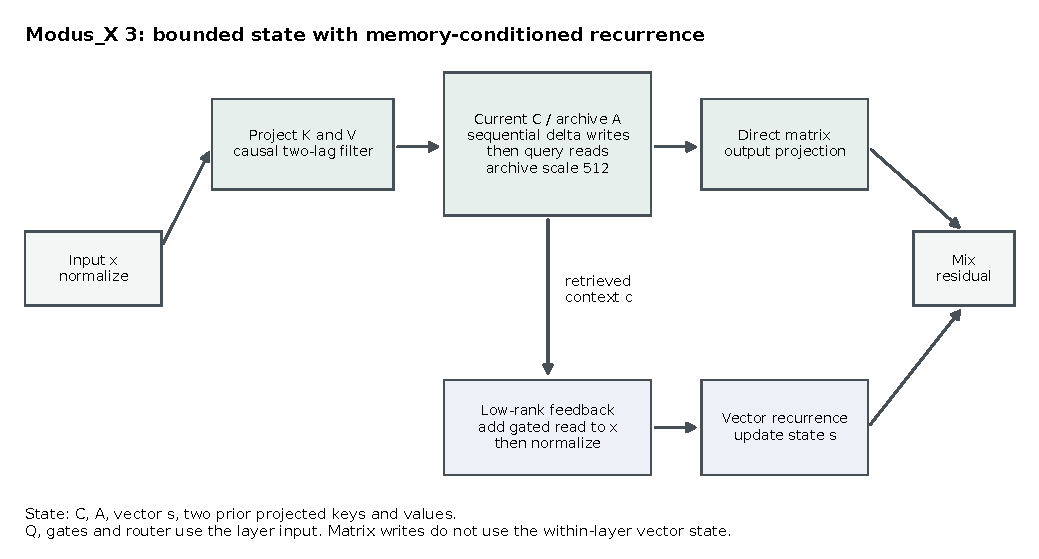
\includegraphics[width=\linewidth]{../figures/architecture.pdf}
\caption{The v3 layer. Retrieved matrix context conditions the vector recurrence
\emph{before} its update; it also retains a direct routed output. The two-lag
filter is causal and stores projected K/V history, not a growing attention cache.
The diagram summarizes dependency, not a parallelization of matrix recurrence.}
\label{fig:architecture}
\end{figure}

\subsection{Locally contextualized keys and values}
Set $e_t=\LN(x_t)$, $u_t^K=W_K e_t$, and $u_t^V=W_V e_t$. For $P\in\{K,V\}$,
\begin{align}
 \widetilde u_t^P &= u_t^P + a_1^P\odot u_{t-1}^P
                              + a_2^P\odot u_{t-2}^P, \label{eq:filter}\\
 k_t &= \norm(\widetilde u_t^K),\quad
 v_t=\tanh(\widetilde u_t^V),\quad q_t=\norm(W_Qe_t).
\end{align}
The lag weights are initialized to zero. Thus the candidate's initial function
matches its control, while the extra weights can learn through their gradients.
Filtering occurs \emph{before} key normalization and value nonlinearity. Queries
remain unfiltered. Histories contain the previous unfiltered projections and
are carried through chunk boundaries. Short causal filters are established
mechanisms; the claim here concerns their tested integration and cost, not their
invention.

\subsection{Current and archive writes}
Let $\beta_t=\eta_t w_t$, where both scalar gates lie in $(0,1)$, and let
$a_t$ be an additional archive-write gate. The implemented updates are
\begin{align}
 C_t &= \rho_t^C C_{t-1}
       +\beta_t(v_t-C_{t-1}k_t)k_t^\top, \label{eq:current}\\
 A_t &= \rho_t^A A_{t-1}
       +\beta_t a_t(v_t-A_{t-1}k_t)k_t^\top. \label{eq:archive}
\end{align}
The prediction residual uses the \emph{previous, undecayed} matrix. Moving decay
inside this residual changes the equations and was tested separately, without
promotion. Reads use the updated matrices. Learned, channel-wise read gates
and a learned scalar current/archive mixture produce
\begin{equation}
 c_t=g_t^{\rm read}\odot
       \left[\mu_t\LN(C_tq_t)+(1-\mu_t)\LN(A_tq_t)\right].
\end{equation}
Both memories share the key, query, value and normalization parameter families
in the frozen implementation; the two states and retention/write gates differ.

\subsection{Archive timescale calibration}
The archive retention gate is parameterized as
\begin{equation}
 \rho_t^A=\sig(z_t^A+\log\tau),\qquad \tau=512.
 \label{eq:clock}
\end{equation}
This multiplies the retention odds by $\tau$. At $z_t^A=0$, retention is
$512/513$, rather than $1/2$. The decay-only half-life is approximately 355
updates, not a guarantee of information retention in the presence of writes and
interference. The offset is fixed throughout the reported local K/V comparisons.
With a free learned retention bias, the offset can be absorbed into that bias:
it changes initialization and optimization coordinates, \emph{not the function
class}. We call it retention calibration rather than a new memory-capacity law.

\subsection{Memory-conditioned vector recurrence and routing}
The matrix read modifies the vector input through a rank-32 bridge:
\begin{align}
 f_t &= U\tanh(Dc_t),\qquad
 \widehat e_t=\LN(x_t+\gamma_t f_t),\\
 s_t &= \alpha_t\odot s_{t-1}
           +\delta_t\odot\tanh(W_u\widehat e_t). \label{eq:vector}
\end{align}
The scalar feedback gate $\gamma_t$ depends on $e_t$; vector coefficients
$\alpha_t,\delta_t$ depend on $\widehat e_t$. A selective vector readout and
output gate produce $y_t^V$. In parallel, a gated projection of $[x_t;c_t]$
produces $y_t^M$. The residual layer output is
\begin{equation}
 x_t^{\rm next}=x_t+\pi_t y_t^M+(1-\pi_t)y_t^V.
\end{equation}
The router $\pi_t$ is predicted from $e_t$. The direct matrix path is retained:
removing it and the router hurt the tested simplification endpoint.

\subsection{State size and computational cost}
For $L$ layers the persistent state has $L(2r^2+n+4r)$ FP32 elements, excluding
weights and transient activations. At the reported dimensions this is 25,288,704
bytes per sequence, compared with 25,190,400 without the local histories. The
increment is 98,304 bytes, or 96 KiB. State size is independent of processed
sequence length, but is quadratic in matrix width. Constant-size state does not
mean constant training memory, unlimited recall, or bounded numerical state
norm. Matrix updates and reads cost $O(r^2)$ per token per layer, in addition to
projection costs.

\section{Two-stage execution}
\label{sec:execution}
The original token loop interleaves matrix updates, feedback, vector updates and
routing. Much of its projection work consequently occurs as small operations
inside a sequential loop. The dependency graph supports a different schedule.
Given a layer's input sequence, its projected matrix inputs and gates do not
depend on its vector state. We therefore execute:
\begin{enumerate}
\item Batch the input-dependent projections and gates over a chunk.
\item Scan the current/archive recurrences and emit retrieved contexts.
\item Batch feedback and vector-coefficient projections from those contexts.
\item Scan the vector recurrence and batch the readout and router mixture.
\end{enumerate}
The tested backend uses 32-token chunks and rematerialization during backward
propagation. Both recurrent scans remain sequential in this backend. For exact
arithmetic, equivalence follows by induction: the matrix states and reads agree
token by token because their inputs agree; conditioned on these reads, the
vector states agree by the same argument; hence the routed outputs agree.
Chunking preserves this reasoning when all state components cross the boundary.
Finite-precision operation ordering can differ, so equivalence is checked
numerically rather than asserted as bit identity.

\begin{figure}[ht]
\centering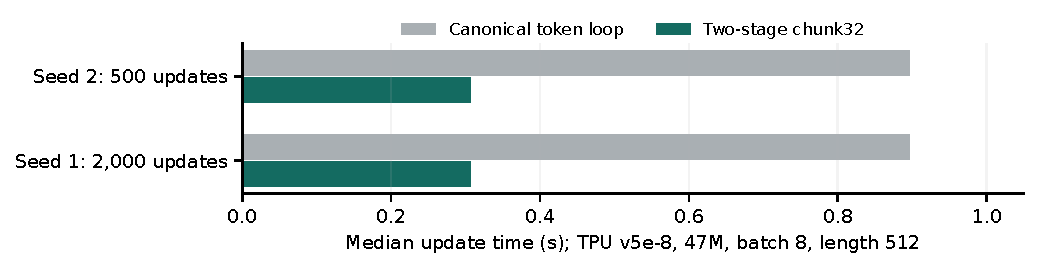
\includegraphics[width=\linewidth]{../figures/execution.pdf}
\caption{Two continuation experiments at 47M parameters. The 2.923$\times$
speedup is median synchronized update time, not whole-job or decoding speed.
Both backends use highest matmul precision.}
\label{fig:execution}
\end{figure}

The first experiment continues seed 2 for 500 updates from step 25,000.
Median update time is 0.896859 seconds for canonical execution and 0.306832
seconds for two-stage execution. Their final dense validation BPC values are
1.432001 and 1.431994, respectively. A second experiment continues seed 1 for
2,000 updates. Update times are 0.897001 and 0.306876 seconds, with validation
BPC 1.421511 and 1.421549. These are two measured continuations, not a claim that
all devices, batch sizes or inference regimes obtain the same speedup.

An earlier independent-trajectory integration check exceeded its strict
0.001 loss-difference threshold at update 14. Subsequent same-state diagnostics
compare both backends at identical parameters and optimizer states: reported
maximum relative gradient error is $3.94\times10^{-6}$ and relative update error
is $6.18\times10^{-7}$. Longer paired language continuation, rather than a
relaxed trajectory assertion, supplies the practical quality check. The failed
integration gate remains in the evidence history.

\section{Experimental design}
\label{sec:protocol}
\textbf{Data and metric.} We use the raw 100,000,000-byte enwik8 file with SHA-256
recorded in the artifact. Training uses bytes $[0,90\mathrm{M})$, validation
$[90\mathrm{M},95\mathrm{M})$, and test $[95\mathrm{M},100\mathrm{M})$.
BPC is mean primary-head negative log likelihood divided by $\log 2$.
Dense evaluation resets state for each 512-byte input window, uses stride 512
at offsets 0 and 256, and includes only complete input/target windows. Each
offset has 9,765 windows per five-million-byte split. Offsets overlap; their
windows are not independent statistical replicates. Sparse 128-window progress
validation is not substituted for dense evaluation.

\textbf{Paired training.} Control and candidate use the same seed-dependent
initial shared parameters, identical random batches and the same optimizer.
Both have archive retention scale 512 and two-stage chunk32 execution. Only the
candidate adds the two-lag K/V filter. Batch size is 8, context 512, and the fixed
endpoint is 25,000 updates, or 102.4M input characters per arm. Training windows
reset recurrent state. AdamW uses weight decay $10^{-4}$, global norm clipping
at 1, LR $6\times10^{-4}$ through step 20,000 and $3\times10^{-4}$ thereafter.
The transition scales the optimizer update while preserving moments and count.

The training objective, measured in nats, is
\begin{equation}
 \mathcal L=\mathcal L_{\rm next}^{(12)}
          +0.05\mathcal L_{\rm next}^{(6)}
          +0.5\mathcal L_{\rm next+1}^{(12)}.
\end{equation}
The last term uses a separate head predicting the byte two positions after the
input byte; its final unavailable target is omitted. It is a training loss, not
future input access. No dropout, label smoothing or auxiliary future-head loss
is enabled in this comparison. Evaluation uses only the primary head.

\textbf{Environment and timing.} Reported runs use Kaggle TPU v5e-8, eight-way
data sharding, JAX 0.10.2, Optax 0.2.8 and highest matmul precision. Timings
synchronize device work and exclude compilation/warmup in their median. They
do not include the entire data preparation, checkpointing and evaluation job.
Control has 47,437,768 parameters; candidate has 47,462,344, an increase of 0.052\%.

\textbf{Protocol chronology.} Seed 1 passed its 5k screen and continued.
Seed 2 failed that screen; after observing seed 1's endpoint, a separately
declared fixed-25k follow-up reran seed 2 from scratch. This is not an additional
independent seed. Seed 3 was prospectively fixed to 25k after the first two
endpoints, with its 5k screen report-only and no quality early stopping. The
three-run series is therefore not described as a wholly preregistered campaign.
Architecture and endpoint schedule were unchanged. Dense validation is the
decision metric; test is evaluated for reporting after that endpoint decision.

\section{Language results and audits}
\label{sec:results}
\begin{table}[ht]
\centering\small\begin{tabular}{crrrrr}
\toprule
Seed & Control val. & MX3 val. & Gain & Control test & MX3 test \\
\midrule
1 & 1.482739 & 1.395448 & 0.087291 & 1.489093 & 1.394951 \\
2 & 1.442483 & 1.432288 & 0.010196 & 1.445116 & 1.432760 \\
3 & 1.427985 & 1.406772 & 0.021213 & 1.431378 & 1.399908 \\
\bottomrule
\end{tabular}

\caption{Frozen 25k paired endpoints. Lower BPC is better; gain is control minus
candidate. Test columns are report-only. The control already includes retention
calibration and the execution backend, so this isolates local K/V filtering.}
\label{tab:endpoints}
\end{table}

The candidate improves dense validation in all three endpoints
(Table~\ref{tab:endpoints}). Gains are 0.087291, 0.010196 and 0.021213 BPC.
Their mean is \MeanGain{}, median \MedianGain{}, and sample standard deviation
\GainSD{}. Mean report-only test gain is \MeanTestGain{} BPC. All three exceed
the frozen 0.005-BPC endpoint threshold. The candidate/control update-time ratios
are 1.001017, 1.001308 and 1.001121, respectively, well below the 1.1 threshold.
These effect sizes support the improvement but do not support a precise
population estimate from only three seeds. We lead with the median as well as
the mean because seed 1 has a much larger effect.

\begin{figure}[ht]
\centering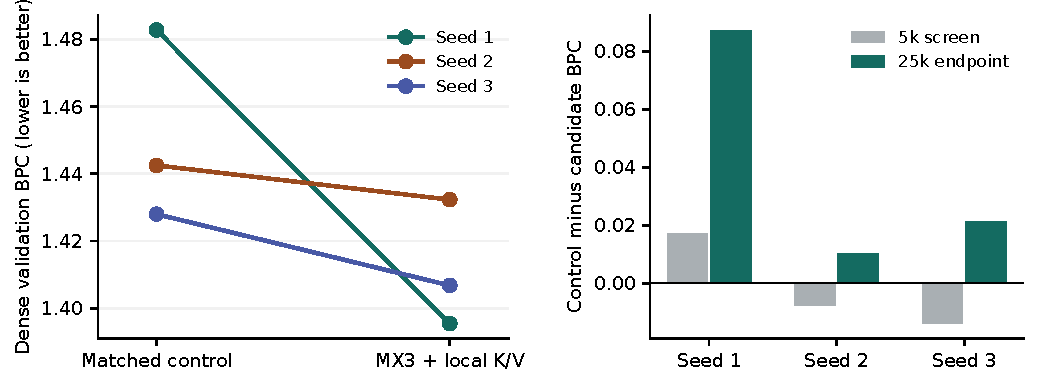
\includegraphics[width=\linewidth]{../figures/endpoints.pdf}
\caption{Paired dense validation endpoints (left) and training-horizon reversal
(right). Seeds 2 and 3 lose their early screens but win at the unchanged 25k
endpoint. The late improvement is observed; its cause is not identified by
these curves alone.}
\label{fig:endpoints}
\end{figure}

\textbf{Checkpoint audits.} Each reported endpoint has a separate read-only
validation audit recording both checkpoint SHA-256 hashes. Reproduced dense
validation differs from the corresponding reported value by at most
$6.85\times10^{-9}$ BPC. Serial/chunk32 comparisons, suffix-causality checks,
streaming handoff and validation reproduction pass for each arm on all three
seeds. The largest reported serial/chunk32 absolute output difference is
$2.29\times10^{-5}$; tested causality and handoff errors are zero. Serial and
chunk32 share the layer equations, so this is an execution audit, not an
independently coded mathematical reference.

\textbf{Carry probes.} Separate probes carry state across the first 65,536
validation targets in one lane. The seed-3 candidate improves from reset BPC
1.396985 to carry BPC 1.346768 on this subset. Both arms benefit from carry on
all three probes. These measurements demonstrate sensitivity to retained state;
they are not the full-split reset metric in Table~\ref{tab:endpoints}, nor a
long-context generalization benchmark.

\section{Connection to prior releases}
\label{sec:history}
The releases~\cite{modus2026} form a sequence of distinct questions, not a single universal
leaderboard. v1.1.1 studied vector/matrix routing and associative retrieval;
v2 introduced current/archive storage and matrix-to-vector feedback; v3 studies
archive calibration, execution efficiency and locally contextualized writes.

\textbf{Retention-only development.} Before local K/V filtering, two development
endpoints compared calibrated retention against recorded MemoryFeedback controls.
Dense validation gains were 0.026833 and 0.006981 BPC, with mean 0.016907 and
approximately unchanged measured runtime. A separate matched streaming closure
on seed 1 improves carry-evaluated validation from 1.410296 to 1.372293 BPC.
The reset and carry protocols are different. Furthermore, the later local K/V
controls do not reproduce the earlier retention-only endpoint values. We retain
both recipe-specific records and do not add their gains, describe a fully crossed
ablation, or infer a v2-to-v3 aggregate from them.

\textbf{Historical language comparison.} At 163.84M processed characters, the
released 81.49M MemoryFeedback model records dense test BPC 1.382445, compared
with 1.384180 for 82.76M \mx{} v1.1.1, 1.345780 for an 81.46M official Mamba
implementation, and 1.419620 for a 76.65M official xLSTM implementation.
These historical endpoints use separate architecture-specific recipes; they
are not parameter-exact controls for the new 47M, 102.4M-character comparison.
Mamba has the stronger compression result in that historical setting. Comparing
its value directly with the v3 table would conflate parameter and training budgets.

\textbf{Controlled memory distinguishes capabilities missed by BPC alone.}
At equal 16,512-byte BF16 inference state, a three-seed v2 clean/update protocol
gives CurrentArchiveDelta 77.95$\pm$1.16\% accuracy and a learned tied-Q/K
Transformer with a 32-token KV window 16.38$\pm$0.75\%. Parameters are 166,791
and 174,112. Clean and overwritten query groups are balanced; latest, previous
and first-value roles are balanced within each group. At a separate larger
64.25-KiB frontier point, the Transformer reaches 98.63\% versus approximately
71.03\% for CurrentArchive. Thus the advantage is a measured low-state-budget
regime, not universal superiority over attention.

An older, single-seed length-128 associative-memory comparison gives
VectorLeanPM 97.325\% versus official Mamba 2.850\% with no overwrite, and
88.850\% versus 3.425\% at 50\% overwrite. Parameters are 145,674 and 162,560.
That large task-specific gap motivates the memory direction; it is not a
three-seed result for the v3 language checkpoint or a comparison with Mamba-3.
The v2 mixed-update task also exposes a weakness: stale false recall on
eligible latest-overwritten queries is 11.28\%, versus 4.65\% for the bounded-KV
Transformer. Better associative storage does not imply perfect version arbitration.

\section{Mechanistic evidence and negative results}
Carrying frozen recurrent state improves prediction in earlier three-seed
audits, with mean full-carry benefit approximately 0.022442 BPC. Matrix and vector
state interventions show that both bodies carry useful information, but do not
establish a strict ``matrix for durable memory, vector for local memory'' division.
Turning off a path at evaluation also changes its input distribution; intervention
regret is not the same quantity as a retrained architecture's performance.

Several plausible changes did not pass their gates. Halving the archive
increased validation BPC by 0.014660, while removing the direct matrix/router path
increased it by 0.063585. Independent erase/write gating lost to the frozen
MemoryFeedback control and added approximately 25\% runtime. Channel-wise
retention and a decay-consistent residual variant did not pass their language
screens. Detached-carry training won on only one of three seeds. These outcomes
motivate preserving the tested core rather than combining failed mechanisms.

\section{Related work and scope of contribution}
Linear attention expresses sequence mixing through fixed-size recurrent
statistics~\cite{katharopoulos2020}. Fast-weight delta updates support targeted
modification of associations~\cite{schlag2021}; DeltaNet develops efficient
sequence-parallel training~\cite{yang2024delta}. Gated DeltaNet combines adaptive
forgetting and delta updates~\cite{yang2024gated}. Kimi Linear's KDA and
Gated DeltaNet-2 further develop channel-wise retention and edit
control~\cite{kimi2025,hatamizadeh2026}. These are relevant prior art, not
mechanisms first introduced by \mx.

Learned recurrent storage also connects to test-time-training layers, whose
hidden state is itself an updated predictive model~\cite{sun2024}, and Titans,
which combines neural long-term storage with short-term attention~\cite{behrouz2025}.
Accordingly, multi-timescale memory and coupling retrieval to prediction are
not claimed as new categories. The present work specifies a particular
two-matrix/vector recurrence, tests its operating-point calibration, and measures
the dependency-preserving execution schedule without adding an attention cache.

Mamba studies selective state-space processing~\cite{gu2023}; xLSTM includes
matrix-memory recurrence~\cite{beck2024}. Mamba-3 explicitly improves retrieval,
state tracking and hardware efficiency~\cite{lahoti2026}. Recent lexical/local
memory designs such as TurboMamba also couple local prediction with a global
recurrent model~\cite{zhang2026}. The present study has no matched v3 comparison
against those newer systems. Associative-recall evaluation is motivated by work
showing that aggregate language loss can hide retrieval failures~\cite{arora2023}.

The contribution of v3 is the specified current/archive-to-vector coordination,
the measured archive-calibration intervention, a dependency-preserving execution
schedule for this layer, and replicated local-filter endpoint evidence under a
fixed state budget. Neither constant-size state, short filtering, gated forgetting
nor matrix delta updates alone is claimed as novel. We do not claim a general
sequence-parallel delta-rule kernel: our tested matrix scan remains sequential.

\section{Limitations and reproducibility}
The new language endpoints cover one byte-level corpus, one model size and
three seeds with development history explicitly disclosed. They establish neither
a fitted scaling law nor useful developer-workload performance. The older Mamba
comparison cannot establish a current cross-family Pareto frontier. No matched
47M Mamba-3, KDA or Gated DeltaNet-2 run is reported. Low-state synthetic memory
results belong to earlier configurations; v3 semantic fact revision and long-form
reasoning remain unmeasured.

The experiment-source commit is
\texttt{766379e89f1395d98b9fc0df3cf4fc7f5a73de6f}.
The companion source and evidence release preserves frozen protocols,
runnable Kaggle cells, negative results, numerical checks and reported checkpoint
hashes. The compact package does not include the large checkpoint payloads.
Result JSONs consolidate recorded runner outputs; the packaging workflow has not
independently downloaded and rehashed those weights. A durable public checkpoint
index, with tested links and recovery files, remains a release-readiness item.
The release scope and remaining checkpoint-hosting checks are explicit in
the release review. The manuscript is licensed CC BY 4.0; software remains MIT.

\section{Conclusion}
\mx{} 3 advances bounded-state language modeling along two separately measured
axes: execution efficiency and predictive quality. Reordering existing dependencies
delivers a 2.923$\times$ update speedup on the tested TPU configuration. Adding
local K/V context then improves all three paired frozen endpoints at approximately
0.12\% mean update overhead, with 96 KiB additional state per sequence.
The resulting model preserves associative matrix storage and memory-conditioned
vector processing without a growing attention cache. The next substantive
comparison is a recipe-matched modern recurrent baseline and a memory-intensive
real workload, rather than another unmatched compression number.

\begin{thebibliography}{14}\footnotesize
\setlength{\itemsep}{1pt}\setlength{\parskip}{0pt}
\bibitem{katharopoulos2020} A. Katharopoulos, A. Vyas, N. Pappas, and F. Fleuret.
Transformers are RNNs: Fast Autoregressive Transformers with Linear Attention.
ICML, 2020. \url{https://arxiv.org/abs/2006.16236}.
\bibitem{schlag2021} I. Schlag, K. Irie, and J. Schmidhuber.
Linear Transformers Are Secretly Fast Weight Programmers. 2021.
\url{https://arxiv.org/abs/2102.11174}.
\bibitem{yang2024delta} S. Yang, B. Wang, Y. Zhang, Y. Shen, and Y. Kim.
Parallelizing Linear Transformers with the Delta Rule over Sequence Length. 2024.
\url{https://arxiv.org/abs/2406.06484}.
\bibitem{yang2024gated} S. Yang, J. Kautz, and A. Hatamizadeh.
Gated Delta Networks: Improving Mamba2 with Delta Rule. ICLR, 2025.
\url{https://arxiv.org/abs/2412.06464}.
\bibitem{kimi2025} Kimi Team. Kimi Linear: An Expressive, Efficient Attention
Architecture. 2025. \url{https://arxiv.org/abs/2510.26692}.
\bibitem{hatamizadeh2026} A. Hatamizadeh, Y. Choi, and J. Kautz.
Gated DeltaNet-2: Decoupling Erase and Write in Linear Attention. 2026.
\url{https://arxiv.org/abs/2605.22791}.
\bibitem{gu2023} A. Gu and T. Dao. Mamba: Linear-Time Sequence Modeling with
Selective State Spaces. 2023. \url{https://arxiv.org/abs/2312.00752}.
\bibitem{beck2024} M. Beck et al. xLSTM: Extended Long Short-Term Memory. 2024.
\url{https://arxiv.org/abs/2405.04517}.
\bibitem{lahoti2026} A. Lahoti, K. Y. Li, B. Chen, C. Wang, A. Bick,
J. Z. Kolter, T. Dao, and A. Gu. Mamba-3: Improved Sequence Modeling using
State Space Principles. ICLR, 2026. \url{https://arxiv.org/abs/2603.15569}.
\bibitem{zhang2026} H. Zhang. TurboMamba: Faster Inference, Faster Training,
and Better Prediction with Lexical Memory. 2026. \url{https://arxiv.org/abs/2610.20682}.
\bibitem{arora2023} S. Arora et al. Zoology: Measuring and Improving Recall in
Efficient Language Models. 2023. \url{https://arxiv.org/abs/2312.04927}.
\bibitem{modus2026} S. Chaudhary. Modus\_X 2.1.0: Coordinated Dual Memory and
Matched Language Scaling. Research software and evidence release, 2026.
\url{https://doi.org/10.5281/zenodo.21590445}.
\bibitem{sun2024} Y. Sun et al. Learning to (Learn at Test Time): RNNs with
Expressive Hidden States. 2024. \url{https://arxiv.org/abs/2407.04620}.
\bibitem{behrouz2025} A. Behrouz, P. Zhong, and V. Mirrokni. Titans: Learning
to Memorize at Test Time. 2025. \url{https://arxiv.org/abs/2501.00663}.
\end{thebibliography}

\appendix
\section{Artifact map and evidence hierarchy}
\small
\begin{tabular}{p{.29\linewidth}p{.64\linewidth}}
\toprule
Artifact & Role \\
\midrule
\texttt{research/v3/01\_*} & Frozen-state interventions, carry probes and failed simplifications. \\
\texttt{research/v3/02\_*} & Archive-timescale screens and over-retention diagnostics. \\
\texttt{research/v3/03\_*} & Retention-only development endpoints and streaming closure. \\
\texttt{research/v3/04\_*} & Backend continuations, numerical checks and frozen execution sources. \\
\texttt{research/v3/05\_*} & Main three-seed K/V protocol, results, checkpoint hashes, sources and cells. \\
\texttt{evidence/} & Prior-release language and controlled-memory evidence; not new v3 trials. \\
\texttt{docs/AGGREGATE.json} & Mechanically calculated paired statistics used in this paper. \\
\texttt{SOURCE\_PROVENANCE.json} & Upstream commit and per-file source hashes. \\
\bottomrule
\end{tabular}
\normalsize

\section{Release and comparison rules}
An arm's state, optimizer moments/count and data RNG belong to the same paired
checkpoint generation. A compact evidence ZIP without those payloads is not a
resumable training artifact. Pickle files must only be loaded from trusted
sources. Raw enwik8 must match the recorded SHA-256 before evaluation; ZIP or
notebook attachment does not guarantee that the dataset is present. Once a
notebook initializes TPU JAX, execution remains in process rather than attempting
to acquire the same accelerator from a second process.

For comparisons, report parameter and persistent-state counts, precision,
hardware, update and character budgets, optimizer/loss settings, and whether
evaluation resets or carries state. Report within-seed differences, not token-level
significance from overlapping windows. Preserve the failed early screens, and do
not select checkpoints, seeds or hyperparameters using report-only test results.
The current package is evidence for its frozen scope, not a pretrained general
assistant or a claim of state-of-the-art language modeling.
\end{document}
